\documentclass[conference]{IEEEtran}
\usepackage{blindtext, graphicx}
\usepackage{hyperref}

% *** GRAPHICS RELATED PACKAGES ***
%
\ifCLASSINFOpdf
  % \usepackage[pdftex]{graphicx}
  % declare the path(s) where your graphic files are
  % \graphicspath{{../pdf/}{../jpeg/}}
  % and their extensions so you won't have to specify these with
  % every instance of \includegraphics
  % \DeclareGraphicsExtensions{.pdf,.jpeg,.png}
\else
  % or other class option (dvipsone, dvipdf, if not using dvips). graphicx
  % will default to the driver specified in the system graphics.cfg if no
  % driver is specified.
  % \usepackage[dvips]{graphicx}
  % declare the path(s) where your graphic files are
  % \graphicspath{{../eps/}}
  % and their extensions so you won't have to specify these with
  % every instance of \includegraphics
  % \DeclareGraphicsExtensions{.eps}
\fi
% graphicx was written by David Carlisle and Sebastian Rahtz. It is
% required if you want graphics, photos, etc. graphicx.sty is already
% installed on most LaTeX systems. The latest version and documentation can
% be obtained at: 
% http://www.ctan.org/tex-archive/macros/latex/required/graphics/
% Another good source of documentation is "Using Imported Graphics in
% LaTeX2e" by Keith Reckdahl which can be found as epslatex.ps or
% epslatex.pdf at: http://www.ctan.org/tex-archive/info/
%
% latex, and pdflatex in dvi mode, support graphics in encapsulated
% postscript (.eps) format. pdflatex in pdf mode supports graphics
% in .pdf, .jpeg, .png and .mps (metapost) formats. Users should ensure
% that all non-photo figures use a vector format (.eps, .pdf, .mps) and
% not a bitmapped formats (.jpeg, .png). IEEE frowns on bitmapped formats
% which can result in "jaggedy"/blurry rendering of lines and letters as
% well as large increases in file sizes.
%
% You can find documentation about the pdfTeX application at:
% http://www.tug.org/applications/pdftex

\hyphenation{op-tical net-works semi-conduc-tor}
\begin{document}
\title{Rating-based Product Recommendation by Collaborative Filtering}

\author{\IEEEauthorblockN{Songxiao Zhang}
\IEEEauthorblockA{Courant Institute of Mathematical\\
Sciences, New York University\\
sz1451@nyu.edu}
\and
\IEEEauthorblockN{Alan Yang}
\IEEEauthorblockA{Courant Institute of Mathematical\\
Sciences, New York University\\
asy233@nyu.edu}
\and
\IEEEauthorblockN{Suzanne McIntosh}
\IEEEauthorblockA{Courant Institute of Mathematical\\
Sciences, New York University\\
sm4971@nyu.edu}}

\maketitle

\begin{abstract}

What determines a good recommendation system?  In the modern society in which electronic commerce or E-commerce is becoming more and more popular and relevant, this becomes an interesting and potentially profitable question.  The main purpose of this project, is for us to explore whether or not we can create a solid recommendation system based on users reviewing certain products and giving these products a high rating.  To accomplish this goal we will be using collaborative filtering, which is a technique commonly used for recommender systems.

There are two approaches to collaborative filtering (CF), namely memory-based CF and model-based CF (Breese et al. 1998). Memory-based CF systems utilize an original, entire user-item rating matrix to generate predictions (Resnick et al. 1994), while model-based CF methods recommend items by first developing a descriptive model of user ratings based on a user-item matrix via different machine learning approaches such as Bayesian network and clustering. The generated model is then used for future prediction about user preferences (Breese et al. 1998). In this paper, we will be looking into these two approaches and evaluating which approach works better for our problem. 

\end{abstract}

\begin{IEEEkeywords}
collaborative filtering, memory-based CF, model-based CF, recommendation system. 
\end{IEEEkeywords}


\section{Introduction}

When consumers shop and browse on big E-commerce sites such as Amazon, they are prompted with other products that they may be interested in.  These products are recommended based on either the consumers search query, or on the consumers previously purchased products.  Amazon even has recommendation systems based on the idea of “Frequently Bought Together” and “Customers Who Bought This Item Also Bought” for whatever product the consumer is currently looking at.  
But what if we want to create a recommendation system that is based on a consumer reviewing a product and rating that product highly.  To be clearer we will consider a specific product “A” as a starting point.  A consumer Bill has reviewed and rated product “A” with five stars.  The next step will be finding all the other users who have given product “A” five stars.  Then all of the products in which these other users have rated five stars will be returned as the recommendation to consumer Bill for review product “A” highly.  (Trimming the returned recommendation list?)

This ideology is based on a technique called collaborative filtering.  Collaborative filtering (CF) is a technique that is highly used for recommender systems.  There are two approaches towards collaborative filtering: memory-based CF and model-based CF (Breese et al. 1998).  Memory-based CF systems utilize an original, entire user-item rating matrix to generate predictions (Resnick et al. 1994), while model-based CF methods recommend items by first developing a descriptive model of user ratings based on a user-item matrix via different machine learning approaches such as Bayesian network and clustering. The generated model is then used for future prediction about user preferences (Breese et al. 1998). In this paper we will discuss and evaluate these two approaches and the results we achieve for our problem.

For this paper, we will only consider review data from Amazon.com and Yelp.com (maybe best buy if we get it).  The data will be collected in bulk and will be preprocessed and used accordingly.  We will process the data so that for each review, we will have the reviewers ID, the review ID, the product ID,  the date, and the rating for the product.


\section{Motivation}


\section{Related Work}

Collaborative Filtering is based on the idea that after analyzing a large amount of information on user preferences, we should be able to predict what the user will like based on similar preferences with other users.

According to \cite{ClusteringItems}, collaborative filtering is most useful in certain situations in which the nearest neighbor model is used for research or commercial systems for generating predictions.  The nearest neighbor model works in three simple phases.  

\begin{enumerate}
  \item The first phase is collecting the appropriate data. This means that the users of whatever system must be able to rate
        items that they have previously experienced. 
  \item The second phase is that the collaborative filtering system will match the user to other participants of the system who
        have similar rating patterns.  This means that the user will share similar interests, opinions, or products as these 
        other participants based on what the collaborative filtering system is used for.  The participants who are closest 
        matched to the original user becomes known as neighbors to the original user, while collectively, all the neighbors 
        form a neighborhood.
  \item Finally, the last step of the model is that the items in which the neighbors have rated highly and the original user has
        never experienced is recommended to the original user.  The items are ranked based on closeness of the neighbor and the 
        consistency of opinion in the neighborhood.
\end{enumerate}

For clarity, if a person “Bob” has the same opinion on an issue as a different person “Alice”, then it is more likely for Bob to share the same opinion on another issue with Alice than with a random different person.  Therefore the issues in which Alice prefers or finds most interesting are the items in which are recommended to Bob.  The example is depicted in Figure 1 below.

\begin{figure}[h]
\centering
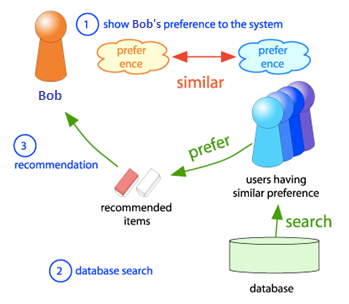
\includegraphics[width=0.5\textwidth]{image/cf_example_flow}
\caption{Example Flow of Collaborative Filtering}
\end{figure}

However, according to \cite{ClusteringItems}, there are some problem that arise with automated collaborative filtering that usually occurs with larger number of items in the prediction domain. These problems are very predictable:

\begin{enumerate}
  \item The first problem is that because users can only buy so many products or listen to so many songs or watch so many
        movies, the density of user ratings on the items available decreases with a larger item set.  Therefore, it becomes 
        less likely that many neighbors will have experienced and share a liking for a specific item as the user.
  \item The second problem is that even though there is a decreased density, the number of items to be considered between 
        each user and their neighbors increases which increases the amount of time necessary to compute the correlations in 
        the neighborhood.
  \item And finally and most importantly as the number of items increases, the items that a user likes becomes more different
        and diverse.  Therefore, it becomes less likely for there to be a correlation between the user’s opinions on a single
        item with all other items available.
\end{enumerate}

These problems make collaborative filtering hard to scale with larger data sets with more items.  These are definitely problems that we are vulnerable to for our project as we do deal with diverse and large item data sets with our Amazon and Yelp data.  O’Connor and Herlocker \cite{ClusteringItems} suggests that a solution is to partition the items based on user rating data.  Partitioning the items will result in fewer items, less ratings, and less users.  The hope is that by clustering together similar items, the prediction accuracy of the collaborative filtering will increase as there may be less noise.  However, although there is potential in certain partitioning algorithms such as kMetis graph partitioning algorithm, the results were that all of the partitioning algorithms resulted in a lower accuracy rate than the un-partitioned collaborative filtering results.  Therefore, our project will not be dealing with partitioning our data into clusters. 

\section{Design}

\subsection{Data Processing}

The review data we will be using for our analysis are from Yelp and Amazon.  The Yelp data was collected from the Yelp Data Set Challenge and Dr. Julian McAuley provided us with the Amazon review data.  The data was originally in JSON format.  Because the data collected are not in the proper structure in which we require, some data processing is required using Pig, Hive and Python.  Hive allows us to create data tables and remove columns in which we consider to be unnecessary.

Firstly, we created tables for each data set using Hive with only the specific columns necessary for our analysis. These  attribute columns are: User ID, Review ID, Rating, Date, and Product ID. The data must then be loaded, filtered, and processed accordingly with Pig so that we have a format which is easy to be used for our data analysis.

\begin{figure}[h]
\centering
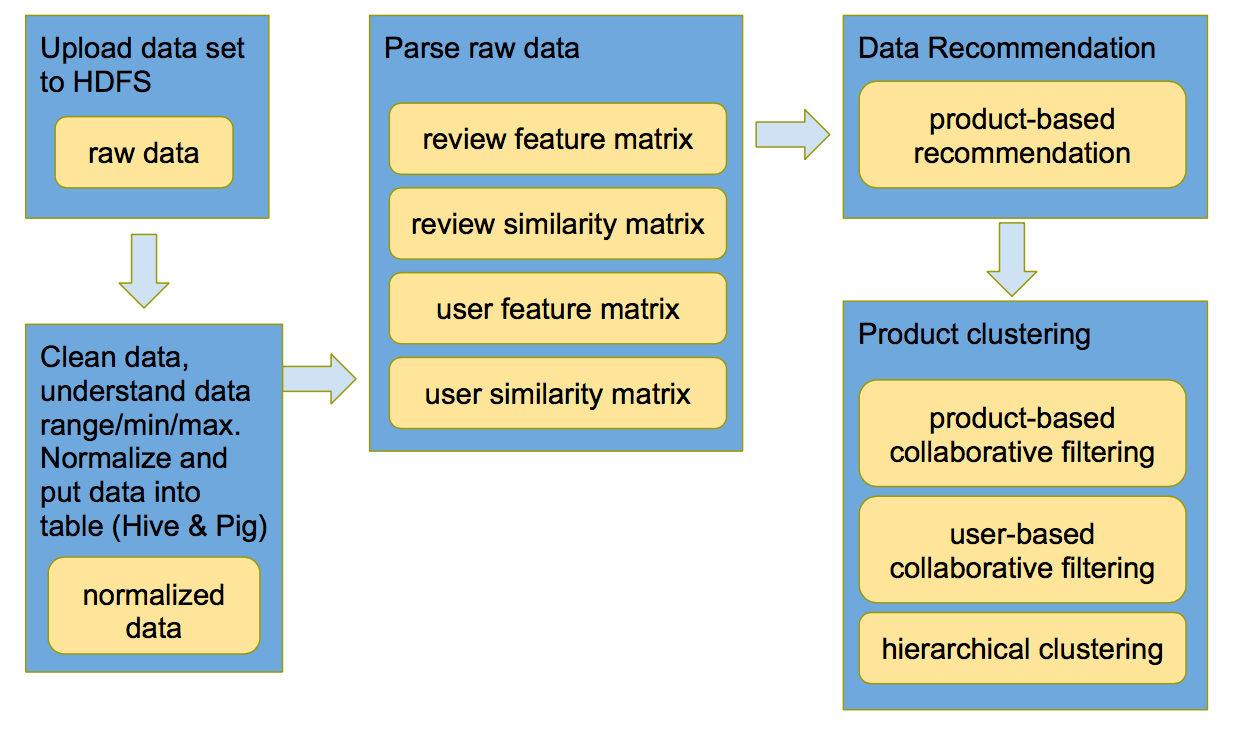
\includegraphics[width=0.5\textwidth]{image/design_diagram}
\caption{Design Diagram on Data Processing to Analysis}
\end{figure}

\subsection{Data Analysis Using Collaborative Filtering}

We will be using Spark and their MLlib to run collaborative filtering.

\section{results}

\subsection{Model Based Collaborative Filtering Results}

\subsection{Memory Based Collaborative Filtering Results}


\section{future work}

\section{Conclusion}




\section*{Acknowledgment}








\begin{thebibliography}{1}

\bibitem{}
Yelp Dataset Challenge, \url{https://www.yelp.com/dataset_challenge}

\bibitem{Image-based}
J. McAuley, C. Targett, J. Shi, A. van den Hengel. Image-based recommendations on styles and substitutes, SIGIR, 2015

\bibitem{substitutable}
J. McAuley, R. Pandey, J. Leskovec. Inferring networks of substitutable and complementary products, Knowledge Discovery and Data Mining, 2015

\bibitem{ClusteringItems}
M. O’Connor, J. Herlocker. Clustering Items for Collaborative Filtering, In: Proceedings of the ACM SIGIR Workshop on Recommender Systems, Berkley, USA, 25-26 August, 1999

\bibitem{Multi-view}
Pradhan, L., Zhang, C., \& Chitrakar, P. (2016). Multi-view Clustering in Collaborative Filtering Based Rating Prediction. 2016 IEEE Tenth International Conference on Semantic Computing (ICSC). $doi:10.1109/icsc.2016.40$

\end{thebibliography}

\end{document}